\documentclass[12pt]{article}
\setlength\parindent{0pt}
\usepackage{fullpage}
\usepackage[margin=0.5in]{geometry}
\usepackage{amsmath}
\usepackage{pdflscape}
\usepackage{xcolor}
\usepackage{graphicx}
\setlength{\parskip}{4mm}
\def\LL{\left\langle}   % left angle bracket
\def\RR{\right\rangle}  % right angle bracket
\def\LP{\left(}         % left parenthesis
\def\RP{\right)}        % right parenthesis
\def\LB{\left\{}        % left curly bracket
\def\RB{\right\}}       % right curly bracket
\def\PAR#1#2{ {{\partial #1}\over{\partial #2}} }
\def\PARTWO#1#2{ {{\partial^2 #1}\over{\partial #2}^2} }
\def\PARTWOMIX#1#2#3{ {{\partial^2 #1}\over{\partial #2 \partial #3}} }
\newcommand{\BE}{\begin{displaymath}}
\newcommand{\EE}{\end{displaymath}}
\newcommand{\BNE}{\begin{equation}}
\newcommand{\ENE}{\end{equation}}
\newcommand{\BEA}{\begin{eqnarray}}
\newcommand{\EEA}{\nonumber\end{eqnarray}}
\newcommand{\EL}{\nonumber\\}
\newcommand{\la}[1]{\label{#1}}
\newcommand{\ie}{{\em i.e.\ }}
\newcommand{\eg}{{\em e.\,g.\ }}
\newcommand{\cf}{cf.\ }
\newcommand{\etc}{etc.\ }
\newcommand{\Tr}{{\rm tr}}
\newcommand{\etal}{{\it et al.}}
\newcommand{\OL}[1]{\overline{#1}\ } % overline
\newcommand{\OLL}[1]{\overline{\overline{#1}}\ } % double overline
\newcommand{\OON}{\frac{1}{N}} % "one over N"
\newcommand{\OOX}[1]{\frac{1}{#1}} % "one over X"

\pagenumbering{gobble}

\begin{document}
\Large

\begin{center}
	Week 13, Day 2 \\
	Exercises on combining rotation and translation
	
	\large
	
	\medskip
	
	Exercise 1: Torque on a yo-yo
	
\end{center}

\normalsize

\begin{minipage}{0.6\textwidth}
A Yo-Yo consists of a cylinder of radius $R$ with a thin slit cut in it. Inside the slit is a smaller inner cylinder of radius $r$ with a string attached to it and then wound around the cylinder. Note that the moment of inertia of a cylinder of radius $R$ is $I=\frac{1}{2}mR^2$; since the slit in the Yo-Yo is so thin, you do not need to consider it in computing the moment of inertia. (Thus, both have the same moment of inertia: $I=\frac{1}{2}mR^2$.)

If a person holds the end of the string and drops the Yo-Yo, it will begin to spin as it falls, unwinding the string as it does. 

\bigskip\bigskip

a) Suppose that you have a red Yo-Yo with $r=0.1 R$ (that is, with a very small inner cylinder) and a blue Yo-Yo with $r=0.4 R$ (with a thicker inner cylinder). Using an argument based on energy, predict which one will fall faster when it is dropped, and describe why it will do so. \textit{(You shouldn't do any calculations here.)}

{\color{red}As they fall, they convert gravitational potential energy to both translational and rotational kinetic energy. The ratio of these is set by the ``no-slip condition'' $v= \omega r_{\rm inner}$ -- in words, the smaller the inner radius, the faster the Yo-Yo must spin to unroll the string as it falls, and the more energy is ``wasted'' as rotation. Thus the red one falls faster.}

\bigskip

{\color{blue}We did this as an example in class. The point here is to get them an intuitive idea of how translation and rotation connect together, while making contact with the previous activity they did in class. The biggest challenge for students in this unit is connecting intuitive ideas framed in words with their mathematical manifestations -- this is the biggest challenge for them throughout our class, but particularly acute here.}
\end{minipage}
\begin{minipage}{0.20\textwidth}
	\begin{center}
		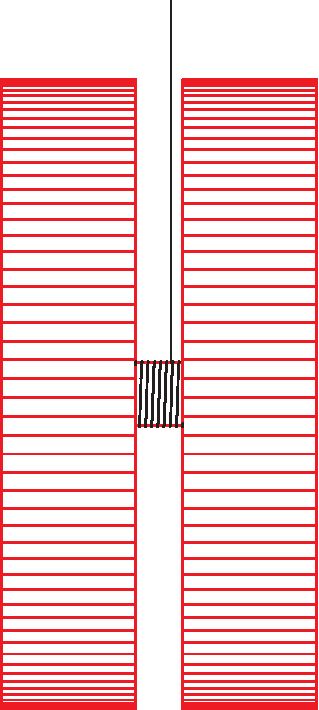
\includegraphics[width=0.7\textwidth]{red-crop.pdf}
		\end{center}
\end{minipage}
\begin{minipage}{0.20\textwidth}
		\begin{center}
		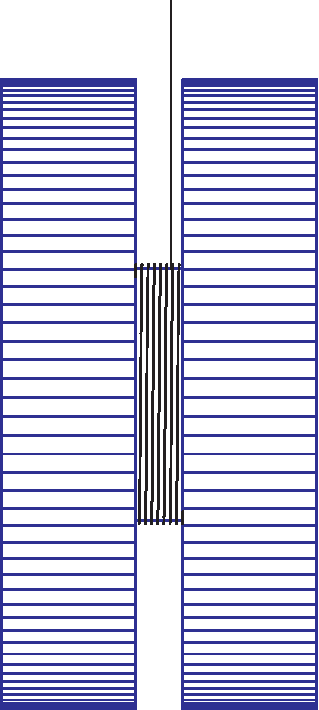
\includegraphics[width=0.7\textwidth]{blue-crop.pdf}
			\end{center}
\end{minipage}


b) Now, you'll calculate the downward acceleration of the Yo-Yo. In this case, the Yo-Yo both {\it translates} and {\it rotates} as it does so.

Start by drawing an extended force diagram for the Yo-Yo, showing all the forces acting on it {\it and where they act}. (Think carefully about which perspective your force diagram should show -- it's not the one in the diagrams above.)

{\color{red}They should make a force diagram as seen from the ``side face'' of the Yo-Yo showing the inner and outer radii (the spool the string is wound around, and the outside of the Yo-Yo.) Gravity acts downward at the center; the tension in the string acts upward at the edge of the inner spool.}

{\color{blue} Students will often try to add other things here, but there are just these two forces. They may need some nudging to see that they can just draw a force diagram cataloguing the forces. You may need to ask them leading questions if they add other spurious forces to get them to realize that they aren't actually present.}



c) Since it both translates and rotates, you will need both $\vec F = m \vec a$ to relate the forces on it to its translational acceleration and $\tau = I \alpha$ to relate the torques on it to its linear acceleration. Construct both of these equations, using the forces that appear on your force diagram. \textit{(Hint: The tension in the string both applies a torque to the Yo-Yo and affects its translational acceleration.)}

{\color{blue} \bf Here there is a significant subtlety dealing with minus signs. \rm I haven't told them whether the string is on the ``left side'' or ``right side'' of the Yo-Yo and it shouldn't matter, but they need to think clearly in analyzing it. The torque from the string will be either clockwise or counterclockwise (depending on how they have drawn their diagrams). Likewise, the relationship between linear and angular acceleration will be $a = \pm \alpha r$, where the sign again depends on how they draw their diagrams and which directions they consider to be positive and which they consider to be negative.}

{\color{red}
	
	Depending on their choice of axes and signs, they will have something like:
	
	\begin{align*}
		T - mg =& ma \\
		Tr =& I \alpha = \frac{1}{2}mR^2 \alpha \\
		\end{align*}
	
}


d) In the above two equations, you will have three unknowns: the tension in the string, the translational acceleration, and the angular acceleration $\alpha$. However, you can relate two of them to each other. What is that relation? \textit{(Hint: Think carefully about minus signs here!)}

{\color{red}
Depending on coordinate system and how they have drawn their yoyo, they will have $a = \pm \alpha r$.
}


e) Now you should have enough information to solve for $a$ in terms of $g$, $r$, and $R$. Once you have a value for your acceleration, call your GTA or coach over and have them check your work. Discuss with them whether the red or blue Yo-Yo in part (a) would fall faster. 

{\color{blue}They may be intimidated by this, but it is the same sort of system of equations that they have had earlier in the semester. They will need to substitute the ``no-slip'' condition in to the rotational equation and then solve.}

{\color{red}
	
	For my choice of coordinates (up is positive, counterclockwise is positive, string on right):
		\begin{align*}
		T - mg =& ma \\
		Tr =& I \alpha = \frac{1}{2}mR^2 \alpha \\
		a =& - \alpha r
	\end{align*}

we substitute into the second equation to get 

$$Tr = \frac{1}{2}mR^2 (-a/r)$$

which tells us that 

$$T = -\frac{1}{2}ma \left( \frac{R}{r}\right)^2$$

Gut check here: the minus sign shouldn't surprise us since $a$ is downward, which I am calling positive. Then substitute that into the force equation to get:

$$
-\frac{1}{2}ma \left( \frac{R}{r}\right)^2 - mg = ma
$$

which gives

$$
a = \frac{-g}{1 + \frac{1}{2} \left(\frac{R}{r}\right)^2}
	$$
}

{
\color{blue}

The ``which one falls faster?'' question is there to prompt them to think about this. If there is no string then the acceleration is just $-g$, and the second term in the denominator is the influence of the added rotational inertia. We can see in it the remnants of the moment of inertia ($\frac{1}{2} = \lambda$) and the substitutions we have made for the no-slip condition. It will fall slowest if the denominator is larger; this happens when $R$ is much bigger than $r$.
}

\newpage

\begin{center}
	\large Exercise 2: a Ping-Pong ball on a table
\end{center}

Some people are playing Ping-Pong outdoors and have left a ball of mass $m$ on the table when a gentle breeze begins; this wind applies a constant horizontal force $F_w$ on the ball. The coefficient of static friction between the ball and the table is $\mu_s$, and the coefficient of kinetic friction is $\mu_k$. The Ping-Pong ball is a hollow shell and has a moment of inertia $\frac{2}{3}mr^2$.

\begin{enumerate}

\item Suppose first that the breeze is very gentle, so that the ball rolls smoothly on the table without slipping. If $F_w$ is very small, will the frictional force on the ball be $\mu_s mg$, $\mu_k mg$, or some other value $F_f$ that you don't know yet? Discuss this with your group and call your coach or TA over to join your conversation. {\it (Don't continue here until you've discussed this with one of your instructors.)}

{\color{red}Very important here that they get this: if the wind is very gentle, then the frictional force will only be whatever is necessary to keep the ball's rotation synchronized with its translation. (In the limit as $F_w$ goes to zero, $F_f$ must as well.) Remind them that $\mu_s F_N = \mu_s mg$ is just the {\it maximum} value of static friction, not what it always is. So they should leave $F_f$ as an unknown variable in their equation here, since they don't know what it is yet.}

\bigskip

\item Determine the ball's translational acceleration $a$ and angular acceleration $\alpha$ in terms of $F_w$ and $m$. (You will need to do all the usual things that you did during the last problem -- draw a force diagram, etc.)

{\color{blue}
	
	Here I'm not outlining the steps for them, but they are the same as the previous problem. They will need to draw a force diagram, think about the relationship between translational and rotational quantities, and write down both $F=ma$ and $\tau = I \alpha$. They will as before need to think carefully about plus and minus signs.}

{\color{red}
	
	Choosing right to be positive and the wind to be blowing to the right, we have
	
	\begin{align*}
		F_w - F_f =& ma \\
		-F_f r =& \frac{2}{3}mr^2 \alpha \\
		a = - \alpha r
	\end{align*}

    Substitute the no-slip condition in to the rotation equation, noting that the minus signs on each side cancel:
    
    $$F_f = \frac{2}{3}ma$$
    
     and substitute that into the first equation to get
    
    $$F_w - \frac{2}{3}ma = ma \rightarrow a = \frac{F_w}{\frac{5}{3}m}$$
    
    where once again we see the pattern that the need to make the object rotate makes the inertia bigger than just $m$. (The denominator is $m(1 + \lambda)$.)
    
}
\newpage

\item Now, suppose that the wind steadily increases in strength. What is the largest wind force $F_w$ for which the ball will roll without slipping? {\it (What other force limits how strong the wind can be?)}

{\color{red}
	The wind that doesn't cause skidding is limited by the maximum force of static friction; to find the limiting case, we use the same equations but set $F_f = \mu_s F_N = \mu_s mg$.
	
	This gives from above
	
	$$F_f = \frac{2}{3}ma = \mu_s mg$$
	
	which tells us that
	
	$$a = \frac{3}{2} \mu_s g.$$
	
	Substitute to get
	
	$$F_w - \mu_s mg = \frac{3}{2} \mu_s mg \rightarrow F_w = \frac{5}{2}\mu_s mg.$$


}
	
	
\item Suppose that the wind becomes even stronger, so that the ball skids across the table. Now determine both its translational acceleration $a$ and its angular acceleration $\alpha$.

{\color{blue}
	
	The important thing for the students to realize here is that when the ball is skidding, the rotation and translational accelerations are no longer coupled since the ``no-slip'' condition no longer applies. Now the two accelerations are decoupled and each can be calculated separately.}

{\color{red}
	
	The horizontal forces are kinetic friction pointing backwards and wind pointing forwards:
	
	
	Newton's law for translation gives:
	$$F_w - \mu_k mg = ma \rightarrow a = \frac{F_w - \mu_k mg}{m}$$
	
	And the only force causing a torque is friction:
	
	$$-\mu_k mgr = \frac{2}{3}mr^2 \alpha \rightarrow \alpha = -\frac{2}{3} \frac{\mu_k g}{r}$$
}	

\end{enumerate}


\end{document}
